% !TeX root = ../main_ustc.tex
\chapter{面向人机协同柔性操作的动态仲裁方法}
\label{chap:ch4_human_arbitration}

第~3~章围绕给定参考轨迹下的柔性接触执行问题，建立了力位增广模型和合作博弈控制器。该控制器能够在位置跟踪与接触力调节之间形成可解释折中，但其前提是期望轨迹、期望接触力和安全边界已经给定。实际人机协同柔性操作中，参考轨迹经常需要操作者在线修正。操作者可以根据视觉观察、接触力反馈、材料变形和任务经验给出横向绕行、局部补扫、目标重定向或停止推进等监督输入，这些输入体现了人在复杂柔性环境中的判断能力。物理交互作为任务通信方式的研究也表明，人的纠正往往包含对局部轨迹和任务目标的有效信息\cite{losey2018trajectory,losey2022physicalcommunication}。

人类输入也会给接触安全带来新的不确定性。沿表面切向的修正可能改善扫描覆盖或避开缺陷区域，沿接触法向的压入可能造成过大的接触力，短时抖动和误触也可能被直接映射为机器人参考轨迹。为使第~3~章执行层控制器在有人参与的任务中可靠工作，本章研究参考层动态仲裁方法。该方法把主端输入转换为人侧候选参考，结合接触安全预测和切向、法向分解得到安全参考，再由多因素动态仲裁参数决定人侧安全参考进入最终期望轨迹的程度。本章中 $\alpha_{\mathrm{HR}}$ 表示参考层人机仲裁权重，$\alpha_{\mathrm{FP}}$ 仍专用于第~3~章执行层力位优先级，二者在物理含义和作用层级上保持分离。

\section{柔性接触任务中的人类介入}
\label{sec:ch4_human_intervention}

柔性接触操作的参考轨迹通常由离线规划、视觉引导或工艺路径给出。设机器人末端接触点位置为 $x(t)\in\R^n$，自主参考轨迹为 $x_r(t)\in\R^n$，环境作用于工具的接触力为 $f_e(t)\in\R^n$，受控法向接触力为 $y_f(t)$。接触力需要保持在安全区间 $[F_{\min},F_{\max}]$ 内，期望接触力记为 $F_d$，并满足 $F_{\min}<F_d<F_{\max}$。在给定 $x_r(t)$ 与 $F_d$ 的条件下，第~3~章执行层控制器负责完成力位协同控制；本章关注的对象是操作者输入如何影响参考轨迹。

操作者通过主端设备或手柄给出监督输入，记为
\begin{equation}
  s_h(t)=\left\{\Delta x_m(t),\dot x_m(t),f_m(t)\right\},
  \label{eq:ch4_human_input}
\end{equation}
其中 $\Delta x_m(t)$ 为主端位移增量，$\dot x_m(t)$ 为主端速度，$f_m(t)$ 为主端交互力或等效输入强度。主端输入首先映射为直接遥操作参考 $x_{\mathrm{tele}}(t)$，再与机器人自主参考融合为人侧候选参考 $x_h(t)$。候选参考经过接触安全投影后得到人侧安全参考 $x_h^{\mathrm{safe}}(t)$，最终通过人机仲裁权重 $\alpha_{\mathrm{HR}}(t)$ 生成执行层使用的期望轨迹 $x_d(t)$。这些变量均位于参考层，作用是为第~3~章执行层控制器提供连续、有界且具有安全含义的任务参考。

\begin{problem}[柔性接触人机动态仲裁问题]
\label{prob:ch4_hr_arbitration}
给定自主参考轨迹 $x_r(t)$、主端监督输入 $s_h(t)$、接触力安全区间 $[F_{\min},F_{\max}]$ 和第~3~章执行层控制器，设计人侧参考生成、安全参考投影和动态仲裁律，使最终期望轨迹 $x_d(t)$ 满足以下要求：
\begin{enumerate}[label=(\arabic*)]
  \item 安全切向修正能够平滑进入 $x_d(t)$，使操作者对扫描覆盖和局部绕行的监督作用得到保留；
  \item 可能导致接触力越界的法向压入受到削弱，使 $x_d(t)$ 不直接放大危险输入；
  \item 短时扰动和手部抖动经过滤波后保持人机仲裁权重平滑；
  \item $x_d(t)$ 及其变化率在工作区间内有界，从而满足执行层控制器对参考信号的基本要求。
\end{enumerate}
\end{problem}

在上述问题中，内部融合系数 $\beta(t)$ 与最终仲裁权重 $\alpha_{\mathrm{HR}}(t)$ 需要明确区分。$\beta(t)$ 用于把直接遥操作参考与机器人自主参考融合为候选人侧参考，反映操作者输入是否足够形成一个可考虑的参考方向；$\alpha_{\mathrm{HR}}(t)$ 用于决定安全人侧参考进入最终期望轨迹的权重，直接影响执行层看到的任务目标。前者服务于参考生成，后者服务于参考层仲裁。

\section{人侧监督参考生成}
\label{sec:ch4_supervised_reference}

机器人自主参考由任务规划器、候选目标集合或局部环境信息生成，表示机器人在无人干预时希望执行的名义路径。为与第~3~章执行层接口保持一致，本章将其记为 $x_r(t)$；在共享控制相关文献中，同类自主参考也常记为 $x_{\mathrm{auto}}(t)$。对于操作者局部修正，可以借鉴基于物理交互的轨迹变形思想，将短时交互信号解释为对未来局部参考轨迹的修正方向；对于持续目标重定向，可以采用概率意图识别思想，将候选目标后验概率作为自主参考切换依据\cite{jain2020probabilistic}。这些模块在本章中作为监督参考生成接口使用，正文重点放在参考层仲裁和接触安全筛选。

人侧监督参考生成的第一步是把主端位移转换为从端附近的直接参考。设 $K_m\in\R^{n\times n}$ 为主从比例矩阵，则
\begin{equation}
  x_{\mathrm{tele}}(t)=x(t)+K_m\Delta x_m(t).
  \label{eq:ch4_tele_reference}
\end{equation}
式\eqref{eq:ch4_tele_reference}表示操作者希望机器人在当前接触点附近产生的局部修正。$K_m$ 的取值决定主端位移到从端位移的比例，通常需要结合主端工作空间、机器人末端速度上限和柔性材料安全接触范围设置。由于 $x_{\mathrm{tele}}(t)$ 可能包含抖动、延迟和危险法向压入，它只作为候选参考进入后续筛选过程。

为避免短时微小输入频繁改变参考轨迹，先定义人类干预强度
\begin{equation}
  I_h(t)=
  \sat\left(
  w_x\frac{\norm{K_m\Delta x_m(t)}}{d_m}
  +w_v\frac{\norm{K_m\dot x_m(t)}}{v_m}
  +w_f\frac{\norm{f_m(t)}}{f_m^{\max}},
  0,1
  \right),
  \label{eq:ch4_intensity}
\end{equation}
其中 $d_m$、$v_m$ 和 $f_m^{\max}$ 分别为位移、速度和交互力归一化尺度，$w_x,w_v,w_f\ge0$ 为权重，且 $w_x+w_v+w_f=1$。$I_h(t)$ 越接近 $1$，说明操作者当前输入越强；$I_h(t)$ 越接近 $0$，说明主端输入较弱或接近静止。

持续时间特征用于区分短时误触和持续干预。设 $I_{\mathrm{th}}$ 为有效输入阈值，定义归一化持续时间 $T_h(t)\in[0,1]$ 的动态为
\begin{equation}
  \dot T_h(t)=
  \begin{cases}
    \lambda_T\left(1-T_h(t)\right), & I_h(t)\ge I_{\mathrm{th}},\\
    -\lambda_T T_h(t), & I_h(t)<I_{\mathrm{th}},
  \end{cases}
  \label{eq:ch4_duration}
\end{equation}
其中 $\lambda_T>0$ 为持续时间更新速度。该状态在操作者持续输入时逐渐增大，在输入消失后逐渐衰减。相比直接用瞬时输入幅值，$T_h(t)$ 能够让系统对持续意图更加敏感，对短时扰动更加克制。

由直接遥操作参考与自主参考之间的偏离程度可得到候选融合系数。令
\begin{equation}
  d_{\mathrm{dev}}(t)=\norm{x_{\mathrm{tele}}(t)-x_r(t)},
  \label{eq:ch4_dev_distance}
\end{equation}
并定义目标融合系数
\begin{equation}
  \beta_r(t)=
  \frac{1}{1+\exp[-\gamma_{\beta}(d_{\mathrm{dev}}(t)-d_{\mathrm{th}})]},
  \label{eq:ch4_beta_target}
\end{equation}
其中 $d_{\mathrm{th}}$ 为参考偏离阈值，$\gamma_{\beta}>0$ 决定映射斜率。实际融合系数通过一阶滤波生成：
\begin{equation}
  \dot\beta(t)=\lambda_{\beta}\left(\beta_r(t)-\beta(t)\right),
  \quad \beta(t)\in[0,1].
  \label{eq:ch4_beta_filter}
\end{equation}
于是人侧候选参考为
\begin{equation}
  x_h(t)=\beta(t)x_{\mathrm{tele}}(t)+\left(1-\beta(t)\right)x_r(t).
  \label{eq:ch4_human_candidate}
\end{equation}
当操作者输入较弱或偏离自主参考较小时，$x_h(t)$ 接近 $x_r(t)$；当操作者持续给出较明确修正时，$x_h(t)$ 逐渐靠近 $x_{\mathrm{tele}}(t)$。

柔性接触任务还需要判断输入方向。设人类输入对应的从端速度为 $v_h(t)=K_m\dot x_m(t)$，自主参考速度为 $v_r(t)=\dot x_r(t)$，方向一致性定义为
\begin{equation}
  C_h(t)=
  \frac{v_h^{\T}(t)v_r(t)}
  {\norm{v_h(t)}\norm{v_r(t)}+\varepsilon_c},
  \label{eq:ch4_direction_consistency}
\end{equation}
其中 $\varepsilon_c>0$ 用于避免分母为零。$C_h(t)>0$ 表示人类输入大体沿自主路径方向，$C_h(t)<0$ 表示反向或明显偏离，$C_h(t)\approx0$ 往往对应横向修正。横向修正在柔性表面扫描中具有实际意义，操作者可能利用它绕开局部缺陷或扩大覆盖范围；法向修正则需要结合接触力安全状态进行筛选。

\section{接触安全参考投影}
\label{sec:ch4_safe_projection}

人侧候选参考 $x_h(t)$ 只说明操作者希望机器人如何移动，还没有说明该移动是否会破坏接触安全。柔性接触中，切向位移主要改变扫描覆盖，法向位移直接改变压入深度和接触力。为在参考层区分这两类影响，设 $n_c(t)\in\R^n$ 为单位接触法向，定义法向投影矩阵和切向投影矩阵为
\begin{equation}
  P_N(t)=n_c(t)n_c^{\T}(t),
  \quad
  P_T(t)=I-P_N(t).
  \label{eq:ch4_tangent_normal_projection}
\end{equation}
对任意参考修正 $\Delta x$，$P_T\Delta x$ 表示沿接触表面的切向分量，主要影响轨迹覆盖；$P_N\Delta x$ 表示沿接触法向的分量，主要影响接触力。

参考层采用局部线性接触力预测模型判断候选参考是否安全。对候选点 $\bar x$，预测受控接触力为
\begin{equation}
  \hat F(\bar x;t)=y_f(t)+\hat K_e(t)n_c^{\T}(t)\left(\bar x-x(t)\right),
  \label{eq:ch4_force_prediction}
\end{equation}
其中 $\hat K_e(t)$ 为第~3~章环境估计器给出的表观刚度估计。式\eqref{eq:ch4_force_prediction}服务于参考层安全筛选，执行层仍采用第~3~章的柔性接触模型。若候选参考沿压入方向移动，预测接触力升高；若候选参考沿卸载方向移动，预测接触力降低。在高频控制和小步长修正条件下，该近似能够反映参考点变化对接触力边界的直接影响。

接触力到安全边界的归一化裕度定义为
\begin{equation}
  \rho_F(t)=
  \sat\left(
  \frac{
  \min\left\{y_f(t)-F_{\min},F_{\max}-y_f(t)\right\}}
  {(F_{\max}-F_{\min})/2},
  0,1
  \right).
  \label{eq:ch4_force_margin}
\end{equation}
当 $\rho_F(t)$ 接近 $1$ 时，接触力位于安全区间中部附近；当 $\rho_F(t)$ 接近 $0$ 时，接触力接近上下边界。为预留传感器噪声、刚度估计误差和离散控制延迟，引入安全余量 $\Delta_F>0$，并定义安全参考集合
\begin{equation}
  \mathcal X_s(t)=
  \left\{
  \bar x\in\mathcal X_{\mathrm{ws}}
  \middle|
  F_{\min}+\Delta_F\le \hat F(\bar x;t)\le F_{\max}-\Delta_F,\
  e_{\mathrm{gc}}(\bar x)\le e_{\mathrm{gc}}^{\max}
  \right\},
  \label{eq:ch4_safe_set}
\end{equation}
其中 $\mathcal X_{\mathrm{ws}}$ 为任务工作空间，$e_{\mathrm{gc}}(\bar x)$ 为可选几何约束误差。若任务不包含远心运动或固定通道边界，则式\eqref{eq:ch4_safe_set}中的几何约束项可去掉。对于长工具任务，可令固定点为 $p_c$，工具轴线上一点为 $p_t(\bar x)$，单位轴向为 $a_t(\bar x)$，并取
\begin{equation}
  e_{\mathrm{gc}}(\bar x)=
  \left\|
  \left(I-a_t(\bar x)a_t^{\T}(\bar x)\right)
  \left(p_c-p_t(\bar x)\right)
  \right\|.
  \label{eq:ch4_gc_error}
\end{equation}
该误差表示固定点到工具轴线的距离，用于描述远心运动或固定通道边界的几何偏离。

人侧安全参考由投影问题给出：
\begin{equation}
  x_h^{\mathrm{safe}}(t)=
  \operatorname*{arg\,min}_{\bar x\in\mathcal X_s(t)}
  \norm{\bar x-x_h(t)}^2 .
  \label{eq:ch4_safe_projection}
\end{equation}
该投影选择距离操作者候选意图最近的安全参考。若 $x_h(t)$ 已位于安全集合内，投影基本保留人类输入；若 $x_h(t)$ 可能导致接触力越界，投影会优先削弱危险法向分量，同时尽量保留对扫描覆盖有益的切向修正。

给定人机仲裁权重 $\alpha_{\mathrm{HR}}(t)$ 后，最终期望轨迹定义为
\begin{equation}
  x_d(t)=x_r(t)
  +\alpha_{\mathrm{HR}}(t)P_T(t)\left(x_h^{\mathrm{safe}}(t)-x_r(t)\right)
  +\alpha_{\mathrm{HR}}(t)\kappa_N(t)P_N(t)\left(x_h^{\mathrm{safe}}(t)-x_r(t)\right),
  \label{eq:ch4_final_reference}
\end{equation}
其中 $\kappa_N(t)\in[0,1]$ 为法向输入抑制系数，可由接触力裕度生成，例如
\begin{equation}
  \kappa_N(t)=
  \sat\left(\kappa_{\min}+\left(1-\kappa_{\min}\right)\rho_F(t),
  \kappa_{\min},1\right),
  \quad 0\le\kappa_{\min}\le1 .
  \label{eq:ch4_normal_gain}
\end{equation}
当接触力远离边界时，$\kappa_N(t)$ 较大，系统允许适度法向修正；当接触力接近边界时，$\kappa_N(t)$ 降低，最终参考主要保留切向修正。这样处理使人的局部经验能够影响扫描路径，同时降低危险法向压入对接触力的影响。

\section{多因素动态仲裁设计}
\label{sec:ch4_dynamic_arbitration}

安全投影给出了人侧候选参考的可行版本，但仍需要确定该安全参考在最终期望轨迹中的权重。人机仲裁权重应同时反映操作者意图强度、输入持续性、输入方向和接触安全状态。触觉共享控制和医疗共享控制研究均强调控制权平滑转移的重要性，系统既要让操作者感到自己仍在控制回路中，也要降低瞬时输入造成的权重突变\cite{abbink2011hapticshared,su2022activityaware}。基于这一考虑，本章采用绝对通道和增量通道相结合的动态仲裁结构。

用于仲裁的主要特征包括干预强度 $I_h(t)$、持续时间 $T_h(t)$、方向一致性 $C_h(t)$ 和安全风险 $R_s(t)$。其中前三者已在\cref{sec:ch4_supervised_reference}中定义。安全风险由接触力裕度、法向输入量和可选几何约束误差共同描述：
\begin{equation}
  R_s(t)=
  \sat\left(
  w_F\left(1-\rho_F(t)\right)
  +w_N\frac{\norm{P_N(t)(x_h(t)-x_r(t))}}{d_N}
  +w_G\frac{e_{\mathrm{gc}}(x_h(t))}{e_{\mathrm{gc}}^{\max}},
  0,1
  \right),
  \label{eq:ch4_safety_risk}
\end{equation}
其中 $d_N$ 为法向位移归一化尺度，$w_F,w_N,w_G\ge0$ 为权重。无几何约束任务中可取 $w_G=0$。$R_s(t)$ 越大，表示人侧输入与当前接触安全边界越接近，参考层应更加保守。

方向一致性主要用于解释操作者输入与自主路径的关系。横向修正通常对应局部绕行或补扫需求，应交给切向投影尽量保留；明显反向输入往往意味着任务目标或局部路径存在较大分歧，需要提高仲裁过程的谨慎程度。为使规则库保持低维且可解释，本文将方向一致性作为安全风险的修正项，并将模糊推理核心保持为三输入结构。定义
\begin{equation}
  D_c(t)=\sat\left(R_s(t)+w_C[-C_h(t)]_+,0,1\right),
  \quad [\eta]_+=\max\{\eta,0\},
  \label{eq:ch4_contact_risk_input}
\end{equation}
其中 $D_c(t)$ 表示用于仲裁的综合接触风险，$w_C\ge0$ 为反向输入修正权重。若操作者输入与自主方向相近，则 $D_c(t)$ 主要由接触力裕度和法向压入风险决定；若操作者持续给出反向修正，则 $D_c(t)$ 增大，使仲裁权重的变化更加平缓。

本章采用双通道模糊推理系统（Fuzzy Inference System, FIS）实现动态仲裁。该设计继承了原有长工具共享控制中的仲裁思想：绝对通道回答当前人侧权重应达到的水平，增量通道回答该权重此刻应上升、保持或下降。与单一阈值或单一 S 型映射相比，这种结构把交互幅值、持续性和风险状态同时纳入判断，能够区分短时扰动、持续修正和风险接近边界这几类不同情况。

模糊逻辑控制器的输入首先由连续物理量缩放到规则库使用的论域。令
\begin{equation}
  F_h^{\mathrm{fis}}(t)=s_F I_h(t),\quad
  T_h^{\mathrm{fis}}(t)=s_T T_h(t),\quad
  D_r^{\mathrm{fis}}(t)=s_D D_c(t),
  \label{eq:ch4_fis_inputs}
\end{equation}
其中 $F_h^{\mathrm{fis}}$ 表示进入模糊规则的干预强度，$T_h^{\mathrm{fis}}$ 表示进入模糊规则的持续时间，$D_r^{\mathrm{fis}}$ 表示进入模糊规则的风险相关距离或综合接触风险。实验中取 $s_F=2\,\mathrm{N}$、$s_T=6\,\mathrm{s}$、$s_D=0.1\,\mathrm{m}$，从而使三类输入分别落入 $[0,2]$、$[0,6]$ 和 $[0,0.1]$ 的有效范围。若 $s_F$ 取值较小，同样的人类输入会更早进入中、高强度模糊等级，仲裁权重上升更快；若 $s_T$ 取值较大，持续时间需要更长才能被判定为稳定意图；若 $s_D$ 取值较小，接触风险或空间接近程度对仲裁器的影响会提前出现。

对任意输入变量 $\zeta$，模糊化过程计算其属于各语言等级的隶属度。中间等级采用三角形隶属函数
\begin{equation}
  \mu_{\mathrm{tri}}(\zeta;a,b,c)=
  \begin{cases}
    0, & \zeta\le a\ \text{或}\ \zeta\ge c,\\
    \dfrac{\zeta-a}{b-a}, & a<\zeta\le b,\\
    \dfrac{c-\zeta}{c-b}, & b<\zeta<c ,
  \end{cases}
  \label{eq:ch4_tri_mf}
\end{equation}
两端等级采用左梯形或右梯形隶属函数，以保证变量接近论域边界时仍有稳定的语言解释。绝对通道中，$F_h^{\mathrm{fis}}$、$T_h^{\mathrm{fis}}$ 和 $D_r^{\mathrm{fis}}$ 均使用小、中、大三个等级，分别记为 PS、PM 和 PL；输出 $\lambda_{\mathrm{abs}}$ 使用 Z、PS、PM、P 和 PL 五个等级，表示从接近机器人自主到更偏向人侧安全参考的连续变化。增量通道中，$\dot F_h^{\mathrm{fis}}$、$\dot T_h^{\mathrm{fis}}$ 和 $\dot D_r^{\mathrm{fis}}$ 使用负、零、正三个等级，输出 $\Delta\lambda_{\mathrm{inc}}$ 使用 NL、N、Z、P 和 PL 五个等级，表示权重明显降低、降低、保持、升高和明显升高。

每条模糊规则对应一个三元输入组合。以绝对通道为例，第 $\ell$ 条规则可写为
\begin{equation}
  \mathcal R_{\ell}:\
  \text{若 }F_h^{\mathrm{fis}}\text{ 属于 }A_{\ell},\
  T_h^{\mathrm{fis}}\text{ 属于 }B_{\ell},\
  D_r^{\mathrm{fis}}\text{ 属于 }C_{\ell},
  \text{ 则 }\lambda_{\mathrm{abs}}\text{ 属于 }O_{\ell}.
  \label{eq:ch4_fuzzy_rule}
\end{equation}
规则激活度采用最小算子计算：
\begin{equation}
  \omega_{\ell}=
  \min\left\{
  \mu_{A_{\ell}}(F_h^{\mathrm{fis}}),
  \mu_{B_{\ell}}(T_h^{\mathrm{fis}}),
  \mu_{C_{\ell}}(D_r^{\mathrm{fis}})
  \right\}.
  \label{eq:ch4_rule_activation}
\end{equation}
同一输出等级下的多条规则再通过最大算子聚合。设聚合后的输出隶属函数为 $\mu_{\lambda}(y)$，则绝对通道采用重心法解模糊：
\begin{equation}
  \lambda_{\mathrm{abs}}=
  \frac{\int_0^1 y\,\mu_{\lambda}(y)\,\dd y}
  {\int_0^1 \mu_{\lambda}(y)\,\dd y}.
  \label{eq:ch4_centroid_abs}
\end{equation}
增量通道采用相同的模糊化、规则激活和解模糊过程，只是输出论域换为 $[-0.5,0.5]$：
\begin{equation}
  \Delta\lambda_{\mathrm{inc}}=
  \frac{\int_{-0.5}^{0.5} y\,\mu_{\Delta\lambda}(y)\,\dd y}
  {\int_{-0.5}^{0.5} \mu_{\Delta\lambda}(y)\,\dd y}.
  \label{eq:ch4_centroid_inc}
\end{equation}
由此可见，模糊逻辑控制器通过隶属函数重叠和重心解模糊生成连续仲裁量。隶属函数的重叠宽度决定过渡是否平滑，规则后件决定不同输入组合下的权重倾向，输出等级的分布决定仲裁参数变化幅度。

绝对通道根据当前特征直接给出目标权重水平：
\begin{equation}
  \lambda_{\mathrm{abs},k}=
  \mathcal F_{\mathrm{abs}}\left(
  F_{h,k}^{\mathrm{fis}},
  T_{h,k}^{\mathrm{fis}},
  D_{r,k}^{\mathrm{fis}}
  \right).
  \label{eq:ch4_abs_channel}
\end{equation}
其中 $F_{h,k}^{\mathrm{fis}}$ 描述操作者输入强弱，$T_{h,k}^{\mathrm{fis}}$ 描述该输入是否具有持续性，$D_{r,k}^{\mathrm{fis}}$ 描述当前人侧参考与接触安全边界之间的关系。规则库的基本趋势为：输入强度越大、持续时间越长，$\lambda_{\mathrm{abs}}$ 越倾向增大；当 $D_{r,k}^{\mathrm{fis}}$ 增大时，仲裁器认为当前任务状态与风险边界或局部分歧更加相关，持续而明确的人类修正更容易进入中高权重区域。安全投影和法向抑制系数同时工作，使高权重主要作用于安全人侧参考，危险法向压入在参考层被削弱。

图\ref{fig:ch4_fuzzy_absolute}给出了绝对仲裁通道的隶属函数和控制曲面。图中 $F_h$ 对应本章中的干预强度输入，$D_r$ 对应原有长工具任务中的空间风险记号，在柔性接触任务中由综合接触风险 $D_c$ 承担相同作用。控制曲面固定 $D_r=0.03\,\mathrm{m}$，展示 $F_h$ 与 $T_h$ 对 $\lambda_{\mathrm{abs}}$ 的共同影响。

\begin{figure}[htbp]
  \centering
  \begin{minipage}[t]{0.58\textwidth}
    \centering
    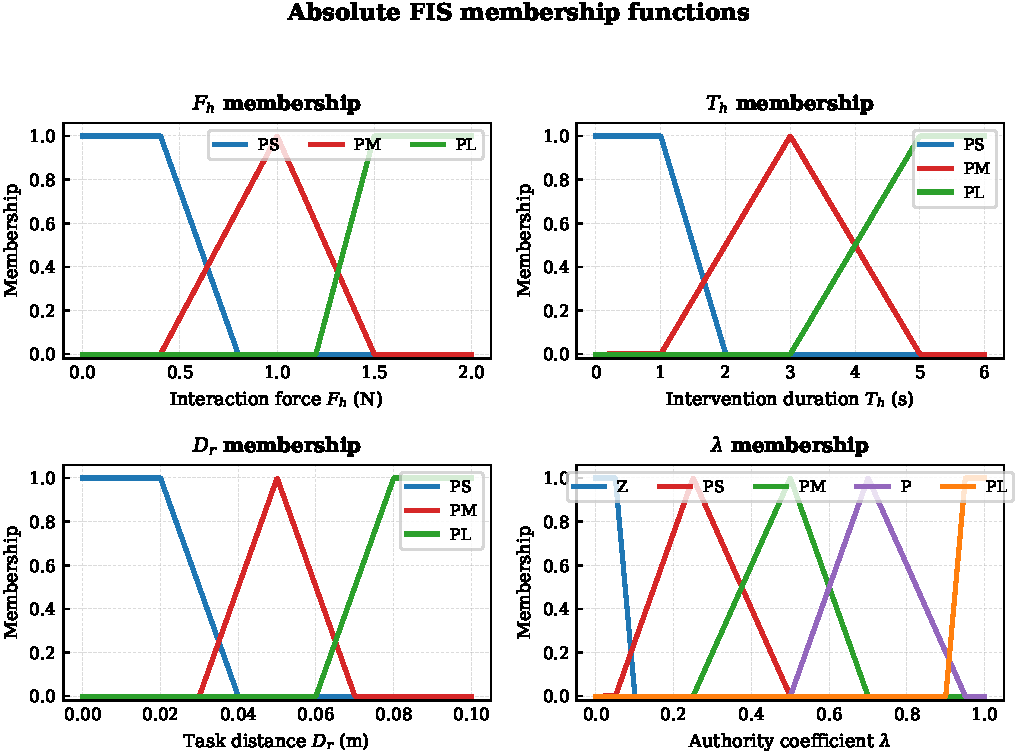
\includegraphics[width=\linewidth]{figures/ch4/fuzzy_logic/fig3a_absolute_membership_ieee.pdf}
  \end{minipage}\hfill
  \begin{minipage}[t]{0.39\textwidth}
    \centering
    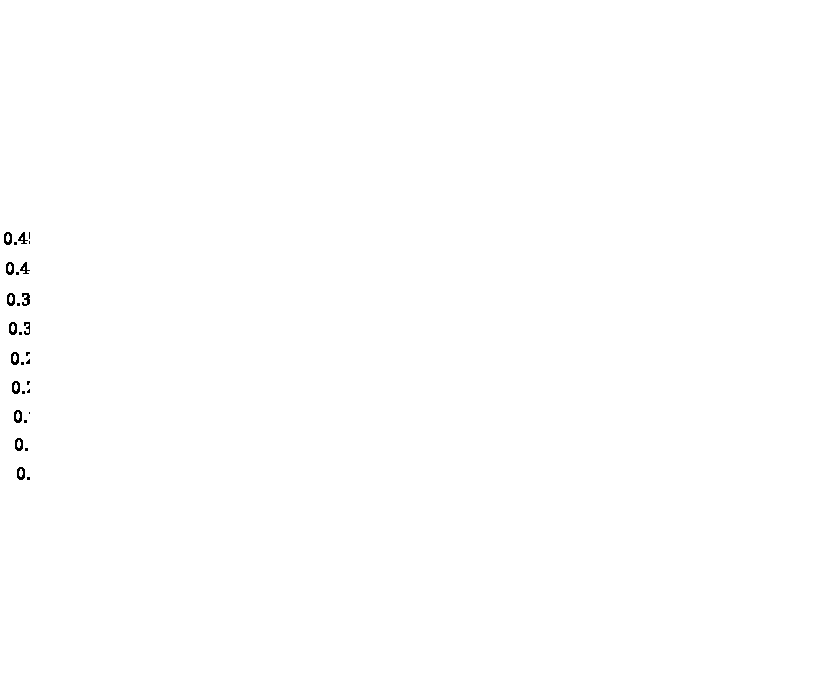
\includegraphics[width=\linewidth]{figures/ch4/fuzzy_logic/fig3b_absolute_surface_ieee.pdf}
  \end{minipage}
  \caption{绝对仲裁通道的隶属函数与控制曲面。}
  \label{fig:ch4_fuzzy_absolute}
\end{figure}

由图\ref{fig:ch4_fuzzy_absolute}可以看出，当干预强度和持续时间均处于低等级时，输出权重位于零或小权重区域，机器人自主参考仍占主导；当操作者持续施加较强输入时，输出逐渐进入中高权重区域，人侧安全参考更容易进入最终期望轨迹。该曲面的斜率变化体现了模糊规则的工程含义：仲裁器对持续而明确的人类意图较敏感，对短时输入保留缓冲空间。

增量通道根据特征变化趋势给出权重调整方向。离散实现中，变化率由相邻采样时刻差分给出：
\begin{equation}
  \dot F_{h,k}^{\mathrm{fis}}=
  \frac{F_{h,k}^{\mathrm{fis}}-F_{h,k-1}^{\mathrm{fis}}}{\Delta t},\quad
  \dot T_{h,k}^{\mathrm{fis}}=
  \frac{T_{h,k}^{\mathrm{fis}}-T_{h,k-1}^{\mathrm{fis}}}{\Delta t},\quad
  \dot D_{r,k}^{\mathrm{fis}}=
  \frac{D_{r,k}^{\mathrm{fis}}-D_{r,k-1}^{\mathrm{fis}}}{\Delta t}.
  \label{eq:ch4_fis_derivatives}
\end{equation}
其中 $\Delta t$ 为采样周期。变化率进入规则库前分别限幅到 $[-3,3]$、$[0,2]$ 和 $[-0.08,0.08]$ 的有效范围。限幅将异常尖峰限制在有效范围内，使单次突变对仲裁结果的影响受控，也使规则库在实验平台采样频率变化时保持可解释性。

\begin{equation}
  \Delta\lambda_{\mathrm{inc},k}=
  \mathcal F_{\mathrm{inc}}\left(
  \dot F_{h,k}^{\mathrm{fis}},
  \dot T_{h,k}^{\mathrm{fis}},
  \dot D_{r,k}^{\mathrm{fis}}
  \right).
  \label{eq:ch4_inc_channel}
\end{equation}
增量通道使用负、零、正三个趋势等级描述输入变化，输出 $\Delta\lambda_{\mathrm{inc}}\in[-0.5,0.5]$ 由明显降低、降低、保持、升高和明显升高五个等级表示。当输入强度和持续时间同时上升、风险趋势平缓时，增量通道推动权重上升；当接触力裕度快速下降、法向压入风险增加或人类输入衰减时，增量通道推动权重下降。绝对通道给出权重的静态位置，增量通道给出权重的运动方向，两者共同使仲裁参数保持连续趋势，减少瞬时查表式跳变。

图\ref{fig:ch4_fuzzy_increment}给出了增量仲裁通道的隶属函数和控制曲面。控制曲面固定 $\dot D_r=0$，用于观察干预强度变化率和持续趋势变化率对 $\Delta\lambda_{\mathrm{inc}}$ 的影响。

\begin{figure}[htbp]
  \centering
  \begin{minipage}[t]{0.58\textwidth}
    \centering
    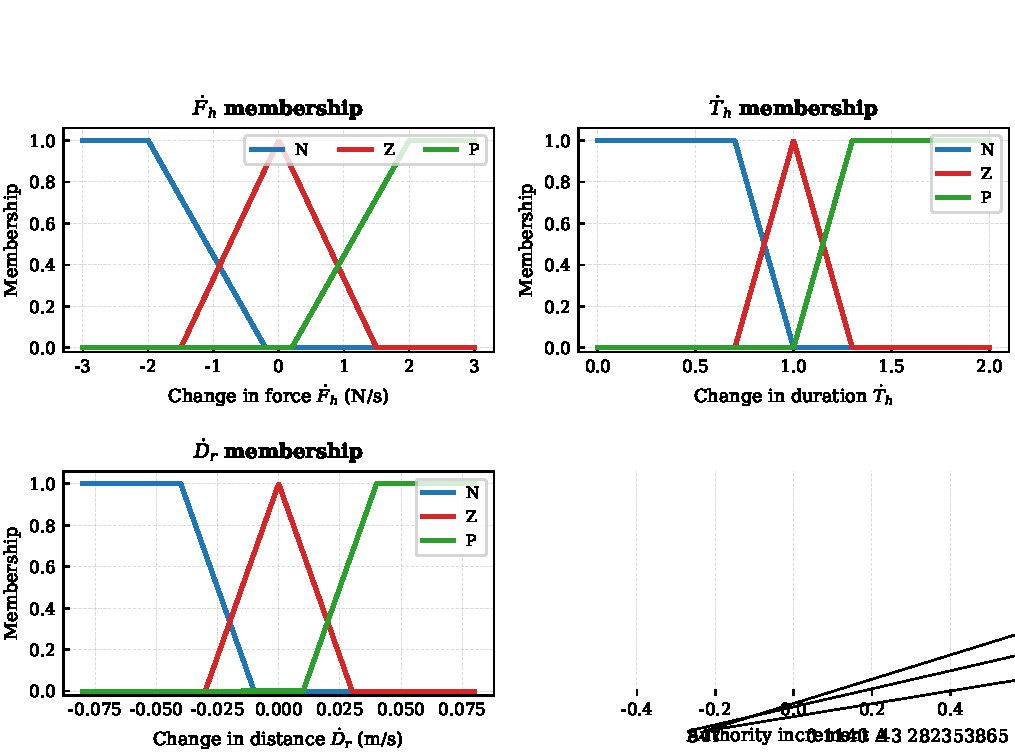
\includegraphics[width=\linewidth]{figures/ch4/fuzzy_logic/fig3c_increment_membership_ieee.pdf}
  \end{minipage}\hfill
  \begin{minipage}[t]{0.39\textwidth}
    \centering
    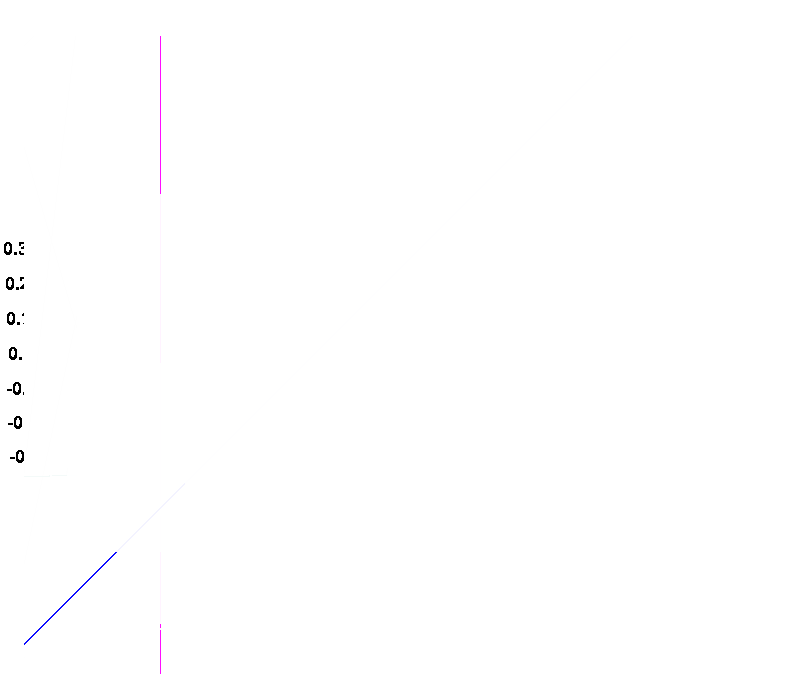
\includegraphics[width=\linewidth]{figures/ch4/fuzzy_logic/fig3d_increment_surface_ieee.pdf}
  \end{minipage}
  \caption{增量仲裁通道的隶属函数与控制曲面。}
  \label{fig:ch4_fuzzy_increment}
\end{figure}

图\ref{fig:ch4_fuzzy_increment}说明，增量通道更关注输入趋势。当干预强度正在增大且持续趋势增强时，$\Delta\lambda_{\mathrm{inc}}$ 取正值，最终权重向人侧安全参考移动；当干预强度下降或持续趋势减弱时，$\Delta\lambda_{\mathrm{inc}}$ 转为负值，系统逐步回到自主参考。对于柔性接触任务，这种趋势判断具有直接意义：操作者刚开始进行局部修正时，权重应逐渐释放；修正结束后，权重应平滑回落，使执行层接收到的期望轨迹保持连续。

增量通道输出先积分为一个权重趋势量：
\begin{equation}
  \lambda_{\mathrm{inc},k}=
  \sat\left(
  \lambda_{\mathrm{inc},k-1}
  +\Delta t\,\Delta\lambda_{\mathrm{inc},k},
  0,1
  \right),
  \label{eq:ch4_inc_integration}
\end{equation}
其中 $\Delta t$ 为仲裁更新周期，$\lambda_{\mathrm{inc},0}$ 通常取 $0.5$。该积分量记录近期权重变化趋势，可理解为增量通道给出的历史一致性判断。为融合绝对权重和增量趋势，定义仲裁状态
\begin{equation}
  \chi_k=
  \begin{bmatrix}
    \lambda_k & \dot\lambda_k
  \end{bmatrix}^{\T},
  \label{eq:ch4_arbitration_state}
\end{equation}
其中 $\lambda_k$ 为离散时刻的未限幅权重估计，$\dot\lambda_k$ 表示其变化趋势。预测模型取
\begin{equation}
  \chi_{k|k-1}=A_f\chi_{k-1|k-1}+B_f\tau_k,
  \quad
  \tau_k=
  \begin{bmatrix}
    \dot\lambda_{\mathrm{abs},k} & \lambda_{\mathrm{inc},k}
  \end{bmatrix}^{\T},
  \label{eq:ch4_filter_predict}
\end{equation}
其中 $\dot\lambda_{\mathrm{abs},k}$ 为绝对通道输出的一阶差分。观测量由绝对权重和增量积分量共同构成：
\begin{equation}
  z_k=
  \begin{bmatrix}
    \lambda_{\mathrm{abs},k} & \lambda_{\mathrm{inc},k}
  \end{bmatrix}^{\T}
  +v_k
  =C_f\chi_k+v_k,
  \label{eq:ch4_filter_measure}
\end{equation}
其中 $v_k$ 表示特征估计噪声。采用常规线性滤波更新
\begin{equation}
  \chi_{k|k}=\chi_{k|k-1}
  +L_k\left(z_k-C_f\chi_{k|k-1}\right),
  \label{eq:ch4_filter_update}
\end{equation}
其中 $L_k$ 为滤波增益。该结构使绝对通道决定当前权重水平，增量通道决定权重变化趋势，滤波器则抑制瞬时噪声和不连续变化。实际实现中，可根据残差滑动窗口自适应调节观测噪声协方差。当绝对通道输出在短时间内剧烈波动，而增量通道给出平稳趋势时，滤波器降低该观测对 $\hat\lambda(t)$ 的影响；当持续输入和风险特征同时保持一致时，滤波器允许权重更快靠近人侧安全参考。这样处理沿用了双通道模糊自适应滤波（Adaptive Kalman Filter, AKF）仲裁的思想，同时把原有空间风险扩展为包含接触力裕度、法向压入和方向分歧的柔性接触风险。

目标人机仲裁权重由限幅得到：
\begin{equation}
  \alpha_{\mathrm{HR},r}(t)=
  \sat\left(\hat\lambda(t),\alpha_{\min}^{\mathrm{HR}},\alpha_{\max}^{\mathrm{HR}}\right),
  \label{eq:ch4_alpha_hr_target}
\end{equation}
其中 $\hat\lambda(t)$ 为滤波后的权重估计。最终权重采用一阶动态生成：
\begin{equation}
  \dot\alpha_{\mathrm{HR}}(t)=
  \lambda_{\mathrm{HR}}\left(
  \alpha_{\mathrm{HR},r}(t)-\alpha_{\mathrm{HR}}(t)
  \right),
  \quad \lambda_{\mathrm{HR}}>0 .
  \label{eq:ch4_alpha_hr_filter}
\end{equation}
$\lambda_{\mathrm{HR}}$ 是人机交互响应速度与参考平滑性之间的调节参数。取值较大时系统更快响应操作者持续输入，但更容易跟随手部抖动；取值较小时期望轨迹更平滑，但操作者可能感到响应迟滞。实际应用中应结合主端采样频率、从端速度限幅和接触材料安全裕度选择该参数。

综合前述参考生成、安全投影和动态仲裁模块，本章方法在每个控制周期内按照“监督参考生成、安全参考投影、意图仲裁、参考输出”的顺序运行。系统先根据主端位移、速度和交互强度生成直接遥操作参考，同时保留机器人自主参考；随后通过参考偏离程度更新 $\beta(t)$，得到人侧候选参考 $x_h(t)$。该步骤将操作者输入先解释为监督参考，再交由后续安全筛选和仲裁模块处理。

在人侧候选参考生成后，系统利用局部力预测模型和安全集合得到 $x_h^{\mathrm{safe}}(t)$，并通过切向和法向投影保留安全切向修正、削弱危险法向压入。接着，系统计算干预强度、持续时间、方向一致性和安全风险，经过绝对通道、增量通道、自适应滤波、限幅和一阶平滑形成最终人机仲裁权重 $\alpha_{\mathrm{HR}}(t)$。最后，式\eqref{eq:ch4_final_reference}生成执行层期望轨迹 $x_d(t)$，由第~3~章力位协同控制器完成接触操作。动态仲裁的作用范围限定在参考层，执行层控制律保持第~3~章的设计。

\section{有界性与可执行性分析}
\label{sec:ch4_boundedness}

本章理论分析服务于一个核心结论：参考层动态仲裁能够向第~3~章执行层控制器提供有界且变化受限的参考输入。为此，需要先说明人侧安全参考投影的存在性，再说明人机仲裁权重的区间不变性，最后把参考层性质与执行层闭环有界性连接起来。

\begin{assumption}[人类输入与自主参考有界]
\label{ass:ch4_input_bounded}
在所考虑的任务工作区间内，自主参考 $x_r(t)$ 及其一阶导数有界，主端输入 $\Delta x_m(t)$、$\dot x_m(t)$ 与 $f_m(t)$ 有界且分段连续。接触法向 $n_c(t)$、表观刚度估计 $\hat K_e(t)$ 和受控接触力 $y_f(t)$ 有界。
\end{assumption}

该假设对应实物系统中的工作空间限制、主端位移限幅、速度限幅和力传感器量程。短时冲击和测量尖峰由输入限幅、低通滤波和硬安全监督处理，并以异常输入事件单独记录。

\begin{assumption}[安全集合非空与局部凸性]
\label{ass:ch4_safe_set}
对每个控制周期，安全参考集合 $\mathcal X_s(t)$ 非空、闭且在当前局部工作区间内凸。若实物系统中因接触力越界或几何约束过紧导致安全集合为空，则参考层退回自主参考 $x_r(t)$，并触发硬安全监督。
\end{assumption}

\begin{lemma}[安全参考投影的存在性与有界性]
\label{lem:ch4_projection_bounded}
在\cref{ass:ch4_input_bounded,ass:ch4_safe_set}成立的条件下，投影问题\eqref{eq:ch4_safe_projection}存在唯一解。若工作空间 $\mathcal X_{\mathrm{ws}}$ 有界，则 $x_h^{\mathrm{safe}}(t)$ 有界；若 $\mathcal X_s(t)$ 随时间分段连续变化，则 $x_h^{\mathrm{safe}}(t)$ 分段连续。
\end{lemma}

\begin{proof}
在有限维欧氏空间中，非空、闭且凸的集合 $\mathcal X_s(t)$ 上，对连续严格凸函数 $\norm{\bar x-x_h(t)}^2$ 求最小值，存在唯一最小点，因此投影问题存在唯一解。又由于 $\mathcal X_s(t)\subseteq\mathcal X_{\mathrm{ws}}$，当工作空间有界时，投影结果 $x_h^{\mathrm{safe}}(t)$ 必然有界。若集合边界和候选参考随时间分段连续变化，度量投影在局部凸集上对参考点保持连续或分段连续，因此 $x_h^{\mathrm{safe}}(t)$ 也分段连续。引理得证。
\end{proof}

\begin{lemma}[人机仲裁权重的区间不变性]
\label{lem:ch4_alpha_hr_invariance}
若 $\alpha_{\mathrm{HR}}(0)\in[\alpha_{\min}^{\mathrm{HR}},\alpha_{\max}^{\mathrm{HR}}]$，且 $\alpha_{\mathrm{HR},r}(t)$ 由\eqref{eq:ch4_alpha_hr_target}生成，则\eqref{eq:ch4_alpha_hr_filter}给出的 $\alpha_{\mathrm{HR}}(t)$ 满足
\begin{equation}
  \alpha_{\mathrm{HR}}(t)\in
  [\alpha_{\min}^{\mathrm{HR}},\alpha_{\max}^{\mathrm{HR}}],
  \quad \forall t\ge0,
  \label{eq:ch4_alpha_hr_interval}
\end{equation}
并且变化率有界：
\begin{equation}
  |\dot\alpha_{\mathrm{HR}}(t)|
  \le
  \lambda_{\mathrm{HR}}
  \left(\alpha_{\max}^{\mathrm{HR}}-\alpha_{\min}^{\mathrm{HR}}\right).
  \label{eq:ch4_alpha_hr_rate}
\end{equation}
\end{lemma}

\begin{proof}
由限幅定义可知 $\alpha_{\mathrm{HR},r}(t)\in[\alpha_{\min}^{\mathrm{HR}},\alpha_{\max}^{\mathrm{HR}}]$。当 $\alpha_{\mathrm{HR}}=\alpha_{\min}^{\mathrm{HR}}$ 时，有 $\dot\alpha_{\mathrm{HR}}\ge0$；当 $\alpha_{\mathrm{HR}}=\alpha_{\max}^{\mathrm{HR}}$ 时，有 $\dot\alpha_{\mathrm{HR}}\le0$。因此该区间为正不变集。进一步，由\eqref{eq:ch4_alpha_hr_filter}可得
\begin{equation}
  |\dot\alpha_{\mathrm{HR}}|
  =
  \lambda_{\mathrm{HR}}
  |\alpha_{\mathrm{HR},r}-\alpha_{\mathrm{HR}}|
  \le
  \lambda_{\mathrm{HR}}
  \left(\alpha_{\max}^{\mathrm{HR}}-\alpha_{\min}^{\mathrm{HR}}\right).
\end{equation}
引理得证。
\end{proof}

\begin{lemma}[最终期望轨迹的有界性]
\label{lem:ch4_reference_bounded}
在\cref{ass:ch4_input_bounded,ass:ch4_safe_set}成立的条件下，若 $x_r(t)$ 有界，$\alpha_{\mathrm{HR}}(t)\in[\alpha_{\min}^{\mathrm{HR}},\alpha_{\max}^{\mathrm{HR}}]$，且 $\kappa_N(t)\in[0,1]$，则由\eqref{eq:ch4_final_reference}生成的最终期望轨迹 $x_d(t)$ 有界。若 $x_r(t)$、$P_T(t)$、$P_N(t)$、$x_h^{\mathrm{safe}}(t)$、$\alpha_{\mathrm{HR}}(t)$ 和 $\kappa_N(t)$ 分段连续，则 $x_d(t)$ 分段连续。
\end{lemma}

\begin{proof}
由\cref{lem:ch4_projection_bounded}可知 $x_h^{\mathrm{safe}}(t)$ 有界，由假设可知 $x_r(t)$ 有界。矩阵 $P_T(t)$ 与 $P_N(t)$ 为正交投影矩阵，其诱导范数不超过 $1$；$\alpha_{\mathrm{HR}}(t)$ 和 $\kappa_N(t)$ 均有界。将这些有界量代入\eqref{eq:ch4_final_reference}可得 $x_d(t)$ 有界。若各组成项分段连续，则有限次加法和乘法保持分段连续性，因此 $x_d(t)$ 分段连续。引理得证。
\end{proof}

\begin{assumption}[执行层对有界参考的实际有界性]
\label{ass:ch4_execution_practical}
第~3~章执行层控制器在有界参考及有界残差作用下具有实际有界性。具体地，存在正定函数 $V(\xi)$ 和正常数 $c_1,c_2,c_3$，使闭环增广状态 $\xi$ 满足
\begin{equation}
  \dot V(\xi)\le
  -c_1\norm{\xi}^2
  +c_2\norm{d(t)}^2
  +c_3\norm{r_d(t)}^2,
  \label{eq:ch4_execution_iss}
\end{equation}
其中 $d(t)$ 为模型残差和外部扰动，$r_d(t)$ 表示由参考轨迹变化率、投影误差和离散更新引入的有界输入项。
\end{assumption}

\begin{theorem}[有界参考下的闭环实际有界性]
\label{thm:ch4_closed_loop_bounded}
若\cref{ass:ch4_input_bounded,ass:ch4_safe_set,ass:ch4_execution_practical}成立，且 $d(t)$ 与 $r_d(t)$ 有界，则采用本章参考层动态仲裁方法和第~3~章执行层控制器构成的闭环系统实际有界。闭环状态最终进入一个有界邻域，该邻域大小与扰动上界、参考变化率上界和安全投影引入的参考修正上界有关。
\end{theorem}

\begin{proof}
由\cref{lem:ch4_projection_bounded,lem:ch4_alpha_hr_invariance,lem:ch4_reference_bounded}可知，参考层生成的 $x_d(t)$ 有界且分段连续，仲裁权重变化率有界。由假设，$d(t)$ 与 $r_d(t)$ 有界，存在 $\bar d,\bar r>0$ 使 $\norm{d(t)}\le\bar d$、$\norm{r_d(t)}\le\bar r$。将其代入\eqref{eq:ch4_execution_iss}可得
\begin{equation}
  \dot V(\xi)
  \le
  -c_1\norm{\xi}^2
  +c_2\bar d^2+c_3\bar r^2 .
  \label{eq:ch4_practical_bound}
\end{equation}
当 $\norm{\xi}^2>(c_2\bar d^2+c_3\bar r^2)/c_1$ 时，$\dot V(\xi)<0$。因此闭环状态最终进入由扰动上界和参考变化上界确定的有界邻域。定理得证。
\end{proof}

\begin{remark}[工程安全边界]
\label{rem:ch4_engineering_safety}
本章的安全参考投影和动态仲裁提供的是参考层连续筛选机制，用于降低危险人类输入进入执行层的可能性。该机制与严格控制屏障函数不同，实物系统仍需要硬力阈值、速度限幅、关节力矩限幅和急停策略。当安全集合为空、接触力超过硬阈值或主端输入异常时，系统应优先执行退回自主参考、停止推进或卸载等工程安全动作。
\end{remark}

通过上述分析可以看到，第四章的作用在于把人类监督输入转化为安全、平滑且可解释的参考轨迹。第~3~章执行层控制器处理给定参考下的力位协同，本章参考层方法处理操作者输入如何进入该参考。后续实验部分将固定执行层控制器，只比较不同参考层仲裁策略对安全切向修正、危险法向压入、短时扰动和持续干预的处理差异。

\section{实验验证}
\label{sec:ch4_experiment}

本节给出动态仲裁方法的仿真与实物实验设置。实验目的集中在参考层，执行层控制器作为固定接口使用。所有实验均采用第~3~章合作博弈力位协同控制器作为固定执行层，期望接触力、安全边界、柔性材料和机器人初始状态在同一组对比中保持一致。不同方法之间只改变人类输入进入最终期望轨迹的方式，从而观察安全切向修正是否被保留、危险法向压入是否被削弱，以及短时扰动是否引起人机仲裁权重突跳。

\subsection{平台设置}
\label{subsec:ch4_platform_setting}

仿真实验采用局部柔性接触模型生成可重复数据，机器人接触点沿柔性表面完成恒力扫描。接触环境设置为低刚度区和高刚度区拼接，并在局部区域加入风险边界，用于模拟材料硬度变化、表面缺陷或任务禁入区域。扫描路径沿切向延伸 $8\,\mathrm{cm}$ 至 $12\,\mathrm{cm}$，扫描速度取 $2\,\mathrm{mm/s}$ 至 $5\,\mathrm{mm/s}$，期望接触力 $F_d$ 取 $0.5\,\mathrm{N}$ 至 $0.8\,\mathrm{N}$，软安全区间可取 $[0.35,1.20]\,\mathrm{N}$。执行层和仲裁层均按 $100\,\mathrm{Hz}$ 更新，每种仿真工况重复不少于 $10$ 次。人类输入由预设时间函数给出，使每一种仲裁策略面对完全相同的输入序列；这一设置便于分离仲裁策略本身的作用，也便于对安全余量、滤波系数和法向抑制系数进行小范围敏感性分析。

实物实验复用现有 Franka 机械臂柔性接触平台。末端安装圆头探针或短接触杆，与硅胶、泡棉或橡胶条等柔性材料接触；主端设备采用 Novint Falcon 或等效手柄输入，必要时使用预设主端输入序列复现相同位移和速度变化。实验前先完成力传感器零偏估计、工具接触点标定和接触法向确认，并根据材料硬度对期望接触力、安全区间和硬安全阈值进行一次性设定。实物记录频率不低于 $100\,\mathrm{Hz}$，每种主要工况重复 $5$ 次左右。主要统计窗口从接触力进入安全区间并保持稳定后开始，接触建立阶段和退出阶段用于观察平台动作连续性。

实物实验定位为平台级重复验证。每组方法在相同初始位姿、柔性材料布置、扫描路径、接触力边界和主端输入尺度下重复运行；控制器参数、模糊隶属函数、参考生成增益和安全投影参数在对比过程中保持一致，参数整定在实验前完成。这样的设置继承了前期主从平台实验的可复现原则，使比较重点集中在参考层仲裁策略对不同人类输入的处理方式。若采用长工具与固定点轴线边界作为补充工况，可沿用简化套管结构和同一主端设备，用于说明仲裁方法在长工具输入下的可执行性；本章主要结论仍以柔性表面接触扫描为对象。

动态仲裁参数采用双通道模糊设置。绝对通道描述当前人侧权重应达到的基础水平，输入为交互强度 $F_h$、有效输入持续时间 $T_h$ 和候选参考相对安全集合的接触风险距离 $D_c$，三个输入的实验范围分别取 $[0,2]\,\mathrm{N}$、$[0,6]\,\mathrm{s}$ 和 $[0,0.1]\,\mathrm{m}$，输出基础人侧权重 $\lambda_{\mathrm{abs}}\in[0,1]$。增量通道描述权重随输入趋势和风险趋势的变化方向，输入 $\dot F_h$、$\dot T_h$ 和 $\dot D_c$ 分别限幅到 $[-3,3]\,\mathrm{N/s}$、$[0,2]$ 和 $[-0.08,0.08]\,\mathrm{m/s}$，输出权重修正量 $\Delta\lambda_{\mathrm{inc}}\in[-0.5,0.5]$。离散实现中，初始权重取 $0.5$，采样周期 $T_s=0.01\,\mathrm{s}$，一阶平滑系数取 $0.9$，最终仲裁权重 $\alpha_{\mathrm{HR}}$ 饱和到 $[0,1]$。主端位移经比例矩阵 $K_m$ 映射为直接遥操作参考，候选融合系数 $\beta$ 由参考偏离程度和一阶滤波生成，安全投影则对候选参考进行切向和法向分解，并根据接触力安全裕度、法向压入趋势和风险距离得到 $x_h^{\mathrm{safe}}$。

绝对通道和增量通道共同决定 $\alpha_{\mathrm{HR}}$ 的变化趋势。当主端输入幅值较小、持续时间较短且风险距离较低时，绝对通道给出较低人侧权重，系统主要跟随自主参考；当操作者持续给出明确切向修正且候选参考仍位于安全区域内时，权重逐步升高，使有效修正进入最终期望轨迹。若输入沿法向压入并导致接触风险上升，安全投影会先削弱危险分量，增量通道也会抑制权重继续升高。由此，模糊仲裁在实验中的作用可以概括为两点：对持续、清晰且安全的监督意图提高接受程度，对短时、突兀或危险的输入降低进入执行层的比例。

\subsection{工况设置}
\label{subsec:ch4_input_setting}

第四章实验围绕四类典型人类输入展开。第一类为安全切向修正，操作者在稳定扫描阶段施加 $10\,\mathrm{mm}$ 至 $20\,\mathrm{mm}$ 的横向偏移，并持续 $3\,\mathrm{s}$ 至 $5\,\mathrm{s}$，用于模拟根据视觉观察或工艺经验调整扫描覆盖区域的情形，主要观察切向修正接受率、轨迹偏移和接触力峰值。第二类为危险法向压入，在 $5\,\mathrm{s}$ 至 $8\,\mathrm{s}$ 的时间窗口内给出 $3\,\mathrm{mm}$ 至 $8\,\mathrm{mm}$ 的法向压入命令，用于模拟误推、过度压入或材料局部凹陷带来的力风险，主要观察法向输入抑制率、力峰值和力越界时间。第三类为短时扰动，输入形式为 $0.2\,\mathrm{s}$ 至 $0.5\,\mathrm{s}$ 的小幅脉冲、反向输入或随机扰动，用于模拟手部抖动、误触和通信尖峰，重点观察仲裁权重峰值、参考突变量和恢复时间。第四类为持续干预，操作者施加 $3\,\mathrm{s}$ 至 $5\,\mathrm{s}$ 的方向一致输入，引导机器人进入新的安全扫描带，主要观察仲裁权重上升时间、轨迹转移平滑性和接触力安全性。

安全切向修正和持续干预主要检验系统对有效人类意图的接受能力。危险法向压入和短时扰动主要检验系统对危险输入和非意图输入的抑制能力。四类输入在仿真中由确定性信号生成，在实物中可先采用预设输入序列重复验证，再由操作者完成少量真实交互试次。真实操作者试次用于说明平台可执行性，正式统计仍以重复性更好的预设输入序列为主。

\subsection{策略设置}
\label{subsec:ch4_method_setting}

对比策略均使用相同执行层控制器和相同安全监督层。无人输入策略取 $x_d=x_r$，操作者输入置零，用于给出机器人自主扫描基线。直接接受策略取 $x_d=x_r+K_m\Delta x_m$，并保留统一硬安全监督，用于显示未筛选人类输入对接触力的影响。固定比例策略使用常数 $\bar\alpha_{\mathrm{HR}}$ 融合人侧候选参考和自主参考，用于观察固定权重对不同输入类型的适应性。单因素仲裁策略由输入幅值或参考偏离程度经 S 型函数生成 $\alpha_{\mathrm{HR}}$，用于检验单一变量对抖动和法向风险的区分能力。无投影仲裁策略依据 $I_h$、$T_h$ 和 $D_c$ 生成动态权重，同时令 $x_h^{\mathrm{safe}}=x_h$，用于分离动态权重与安全参考投影的作用。本章方法同时启用多因素动态仲裁、安全参考投影、切向和法向分解以及权重滤波，用于验证完整参考层仲裁机制。

为保证对比关系清晰，固定比例策略中的 $\bar\alpha_{\mathrm{HR}}$ 在实验前确定，并在所有工况中保持同一取值；单因素仲裁策略使用与本章方法相同的限幅和一阶平滑，输入特征减少为单一变量；无投影仲裁策略保留多因素权重估计，使其与本章方法的差异集中在安全集合投影和法向抑制上。所有策略均使用相同硬安全阈值和速度限幅，硬安全事件单独记录，作为安全边界触发情况报告。参考前期主从平台实验中“同一任务布局、同一参数组、同一输入尺度”的对比原则，本章将对比边界限定在参考层仲裁机制，预测控制与合作博弈执行层的比较归入执行层章节讨论。

\subsection{指标设置}
\label{subsec:ch4_metric_setting}

第四章指标围绕人类输入处理效果设置。切向修正接受率用于衡量有价值的人类横向修正进入最终参考的比例。设 $\mathcal K_T$ 为安全切向修正时间段，则
\begin{equation}
  R_{\mathrm{acc}}=
  \frac{
  \sum_{k\in\mathcal K_T}
  \norm{P_{T,k}(x_{d,k}-x_{r,k})}}
  {
  \sum_{k\in\mathcal K_T}
  \norm{P_{T,k}(x_{h,k}-x_{r,k})}+\varepsilon_m
  },
  \label{eq:ch4_metric_acceptance}
\end{equation}
其中 $\varepsilon_m>0$ 用于避免分母过小。$R_{\mathrm{acc}}$ 越接近 $1$，表示最终期望轨迹越充分保留安全切向修正；若该值过小，说明系统过于保守，操作者有效经验难以进入任务参考。

危险法向输入抑制率用于衡量参考层对过压方向输入的削弱程度。设 $\mathcal K_N$ 为危险法向压入时间段，则
\begin{equation}
  R_{\mathrm{sup}}=
  1-
  \frac{
  \sum_{k\in\mathcal K_N}
  \norm{P_{N,k}(x_{d,k}-x_{r,k})}}
  {
  \sum_{k\in\mathcal K_N}
  \norm{P_{N,k}(x_{h,k}-x_{r,k})}+\varepsilon_m
  } .
  \label{eq:ch4_metric_suppression}
\end{equation}
该指标只在预先定义的危险法向输入窗口内计算。$R_{\mathrm{sup}}$ 越大，说明安全投影、法向抑制系数和动态仲裁共同削弱了更多危险法向参考；若该值过低，则人类法向压入仍可能直接进入执行层。

接触力安全性通过力越界时间和力峰值描述。力越界时间定义为
\begin{equation}
  T_{\mathrm{vio}}=
  T_s\sum_{k=1}^{N}
  \mathbf{1}_{\{y_{f,k}<F_{\min}\ \mathrm{or}\ y_{f,k}>F_{\max}\}},
  \label{eq:ch4_metric_violation}
\end{equation}
其中 $T_s$ 为采样周期，$N$ 为统计窗口内采样点数。力峰值定义为
\begin{equation}
  F_{\mathrm{peak}}=
  \max_{1\le k\le N}|y_{f,k}-F_d|.
  \label{eq:ch4_metric_force_peak}
\end{equation}
$T_{\mathrm{vio}}$ 反映接触力离开软安全区间的持续时间，$F_{\mathrm{peak}}$ 反映最不利瞬间的接触风险。两者共同说明人类输入是否破坏了柔性接触安全。

人机仲裁权重的平滑性用相邻采样差分的均方根值表示：
\begin{equation}
  S_{\alpha}=
  \sqrt{
  \frac{1}{N-1}
  \sum_{k=2}^{N}
  \left(
  \frac{\alpha_{\mathrm{HR},k}-\alpha_{\mathrm{HR},k-1}}{T_s}
  \right)^2
  } .
  \label{eq:ch4_metric_alpha_smoothness}
\end{equation}
$S_{\alpha}$ 越小，说明权重变化越平滑；结合持续干预下的上升时间，可判断系统是否同时具备抑制短时扰动和响应持续意图的能力。轨迹执行质量采用切向轨迹均方根误差辅助评价：
\begin{equation}
  E_T^{\mathrm{RMS}}=
  \sqrt{
  \frac{1}{N}
  \sum_{k=1}^{N}
  \norm{P_{T,k}(x_k-x_{d,k})}^2
  } .
  \label{eq:ch4_metric_tangent_error}
\end{equation}
该指标用于说明执行层是否能够跟随参考层生成的最终期望轨迹。第四章结果分析将优先观察 $R_{\mathrm{acc}}$、$R_{\mathrm{sup}}$、$T_{\mathrm{vio}}$ 和 $F_{\mathrm{peak}}$，再结合 $S_{\alpha}$ 与 $E_T^{\mathrm{RMS}}$ 解释仲裁权重平滑性和轨迹跟随质量。

\subsection{数据处理}
\label{subsec:ch4_data_processing}

每次试验记录时间戳、末端位姿、末端速度、自主参考 $x_r$、人侧候选参考 $x_h$、安全人侧参考 $x_h^{\mathrm{safe}}$、最终期望轨迹 $x_d$、接触力 $y_f$、主端输入、$\beta$、$\alpha_{\mathrm{HR}}$、$D_c$、$\rho_F$、$\kappa_N$ 和单周期计算时间。统计前对力信号进行零偏修正，并使用同一低通滤波窗口处理所有方法的数据。若出现通信中断、硬安全急停、工具未形成有效接触或传感器明显掉线，该试次单独标记并说明原因；正常范围内的力峰值、轨迹误差和主端输入波动保留在统计中。

仿真结果用于展示完整对比趋势和参数敏感性，实物结果用于验证同一仲裁逻辑在真实机械臂、柔性材料和主端输入下的可执行性。结果呈现时，每类工况先给出输入序列和对比策略，再给出轨迹、接触力、仲裁权重和安全投影前后参考的典型时序，最后用均值和标准差汇总主要指标。这样的组织方式使图表分析直接回到本章核心问题：安全切向修正是否进入最终轨迹，危险法向压入是否被削弱，短时扰动是否受到抑制，持续干预是否得到平滑响应。
